The evaluation is divided into three parts: testing, performance, and expressive power. In all parts, Souffle\cite{SouffleHome} is the implementation evaluated against.

\subsection{Testing}
The Souffle pretty-printer (SPP) is used to output a Datalog program that may be executed by Souffle. The process of comparing Souffle output to that of the internal interpreter has been automated and a range of tests written. If the tests agree, then the SPP is said to be correct for the given test program. Assuming that the Souffle result is correct, the internal interpreter too is concluded to be correct for the given test program. The test cases are selected to cover mutual recursion, negation, meta-predicates, and the other various language extensions.

\subsection{Performance}
Souffle implements semi-naive evaluation\cite{Green:2013:DRQ:2688167.2688168} which is essentially the same as naive evaluation except that it utilizes the following key-insight. An instantiation of the terms of a rule may derive new tuple(s) if and only if at least one tuple that was derived in the previous iteration is used in the instantiation. Thus the number of tuples to consider can be greatly decreased. 

The performance is evaluated against two examples shown in figures \ref{figure:nat} and \ref{figure:ancestor}.
\vspace*{-15pt}
\begin{figure}[!ht]
\begin{minipage}[b]{.5\textwidth}
\caption{Upper bounded Natural Numbers example.}
\begin{minted}{text}
Nat(0).
Nat(y) :- Nat(x), BIND(y, x + 1), y <= N.
\end{minted}
\label{figure:nat}
\end{minipage}
\begin{minipage}[b]{.5\textwidth}
\caption{Ancestor relation example.}
\begin{minted}{text}
r1: Ancestor(p, c) :- Parent(p, c).                            
r2: Ancestor(a, c) :- Parent(p, c), Ancestor(a, p).
\end{minted}
\label{figure:ancestor}
\end{minipage}
\end{figure}
\noindent
\vspace*{-15pt}
\subsubsection{Theoretical Prediction}

\paragraph{NAT Example}\NL
For the internal naive algorithm, at step $k$ in the iteration, the $Nat$-relation contains $k$ tuples. The internal implementation uses a tree-set to store the tuples and so each step takes $\mathcal{O}(k \cdot log(k))$ time (there is no join (Appendix A) between Nat and BIND). There are a total of $N$ steps in the algorithm, thus we get the following upper-bound for the worst-case running time:
\begin{align*}
\sum_{k = 1}^{N}k \cdot log (k) \leq N^2 log(N) = \mathcal{O}(N^2 log(N))
\end{align*}
For semi-naive evaluation, each iteration gives a single new element to consider. The corresponding time complexity thus reduces to the order of:
\begin{align*}
	\sum_{k = 1}^{N} log (k) \leq N log(N) = \mathcal{O}(N log(N))
\end{align*}

\paragraph{Ancestor Example}\NL
Assume the initial parent relation: 
\begin{align*}
Parent(P_i, P_{i + 1}), i = 1\ldots N - 1
\end{align*}
\noindent
Then at the $k:th$ iteration of rule $r_2$, the \textit{Ancestor} relation contains $\sum_{l = 1}^{k} (N - l)$ elements. The parent relation is constant with $N$ elements. The dominating (non-indexed) \textit{join}-operation thus has accumulated time complexity:
\begin{align*}
\sum_{k = 1}^{N - 1} \Big (N \cdot \sum_{l = 1}^{k} (N - l)\Big) = \mathcal{O}(N^4)
\end{align*}
\noindent
Similarly, the semi-naive algorithm has expected time-complexity:
\begin{align*}
\sum_{k = 1}^{N - 1} N \cdot (N - k) = \mathcal{O}(N^3)
\end{align*}


\subsubsection{Experimental Results}

\paragraph{NAT Example}\NL
The NAT example was measured for inputs in range 100 to 10000 for the internal evaluation, and in range 4096 to 536870912 for Souffle. The theoretical results was confirmed as $O(N^2 log(N))$ for the internal evaluation. For Souffle, the experimental results show $\mathcal{O}(N)$ behavior. The $log(N)$ does not show in Souffle, most likely due to a more sophisticated relation representation\cite{Scholz:2016:FLP:2892208.2892226}.

%; Souffle better relation data structure as opposed to an ordered set.
%\begin{figure*}%[!ht]
%	\hspace*{-25pt}
%	\begin{minipage}[b]{.5\textwidth}
%		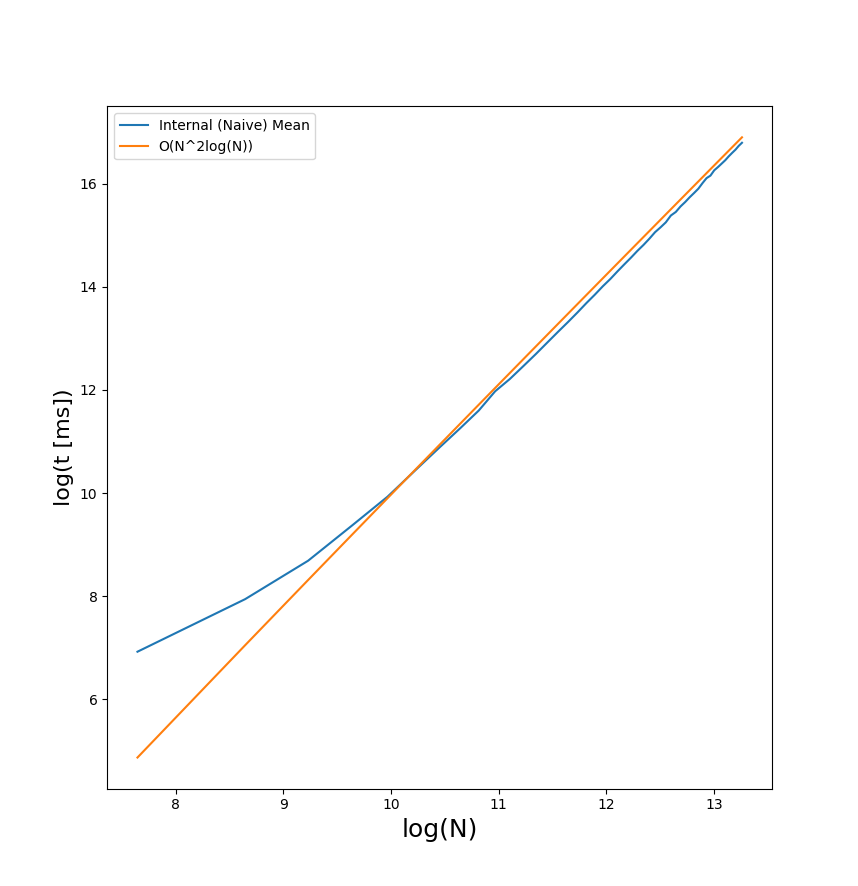
\includegraphics[scale=0.33]{img/internalloglog.png}
%	\end{minipage}%
%	\hspace*{-40pt}
%	\begin{minipage}[b]{.5\textwidth}
%		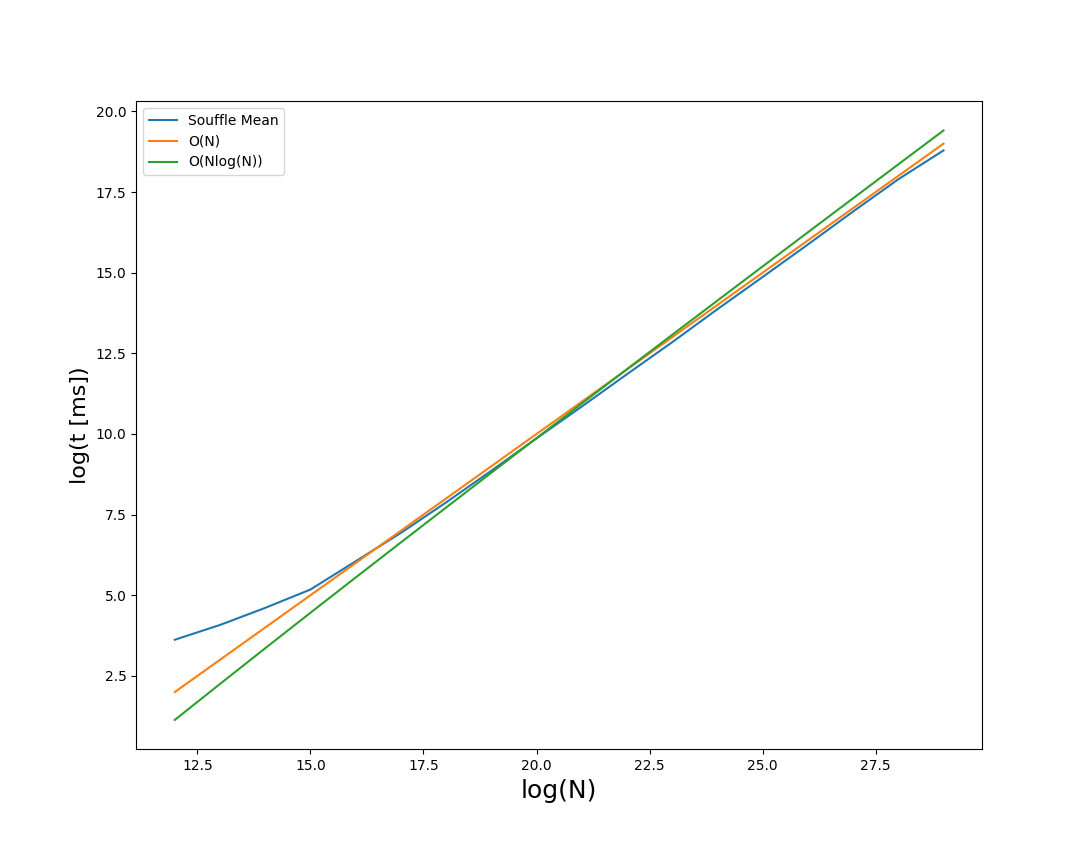
\includegraphics[scale=0.35]{img/souffleloglog.png}
%	\end{minipage}
%	\label{figure:natExperimental}
%	\caption{Nat Example, \textbf{Left: } Internal (Naive), \textbf{Right: } Souffle (Optimized Semi-Naive)}
%\end{figure*}
\paragraph{Ancestor Example}\NL
The ancestor example was measured for inputs in range 5 to 260 for the internal evaluation, and in range 50 to 16384 for Souffle. The theoretical results was again confirmed as $O(N^4)$ for the internal evaluation. Souffle performed better than expected at about $O(N^{2.33})$. Again, this is most likely due to better \textit{join}-performance which can be achieved by storing separate index data structures, thus removing the need to explicitly form the Cartesian product\cite{Scholz:2016:FLP:2892208.2892226}.
%\begin{figure*}%[!ht]
%	\hspace*{-70pt}
%	\begin{minipage}[b]{.5\textwidth}
%		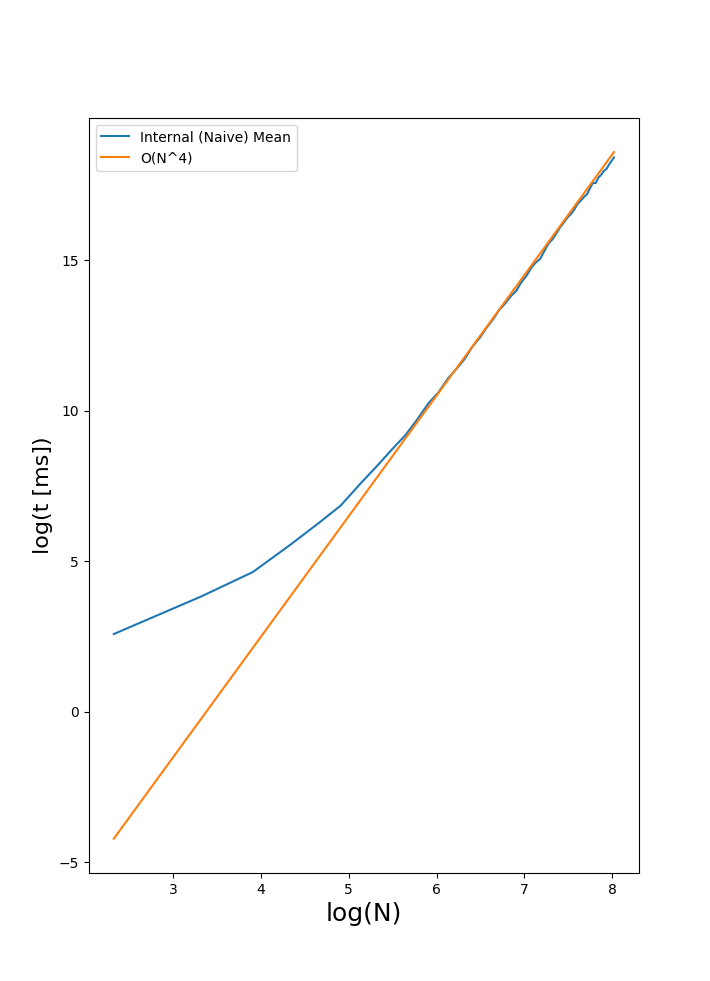
\includegraphics[scale=0.345]{img/ancestorInternal.png}
%	\end{minipage}%
%\hspace*{-70pt}
%	\begin{minipage}[b]{.5\textwidth}
%		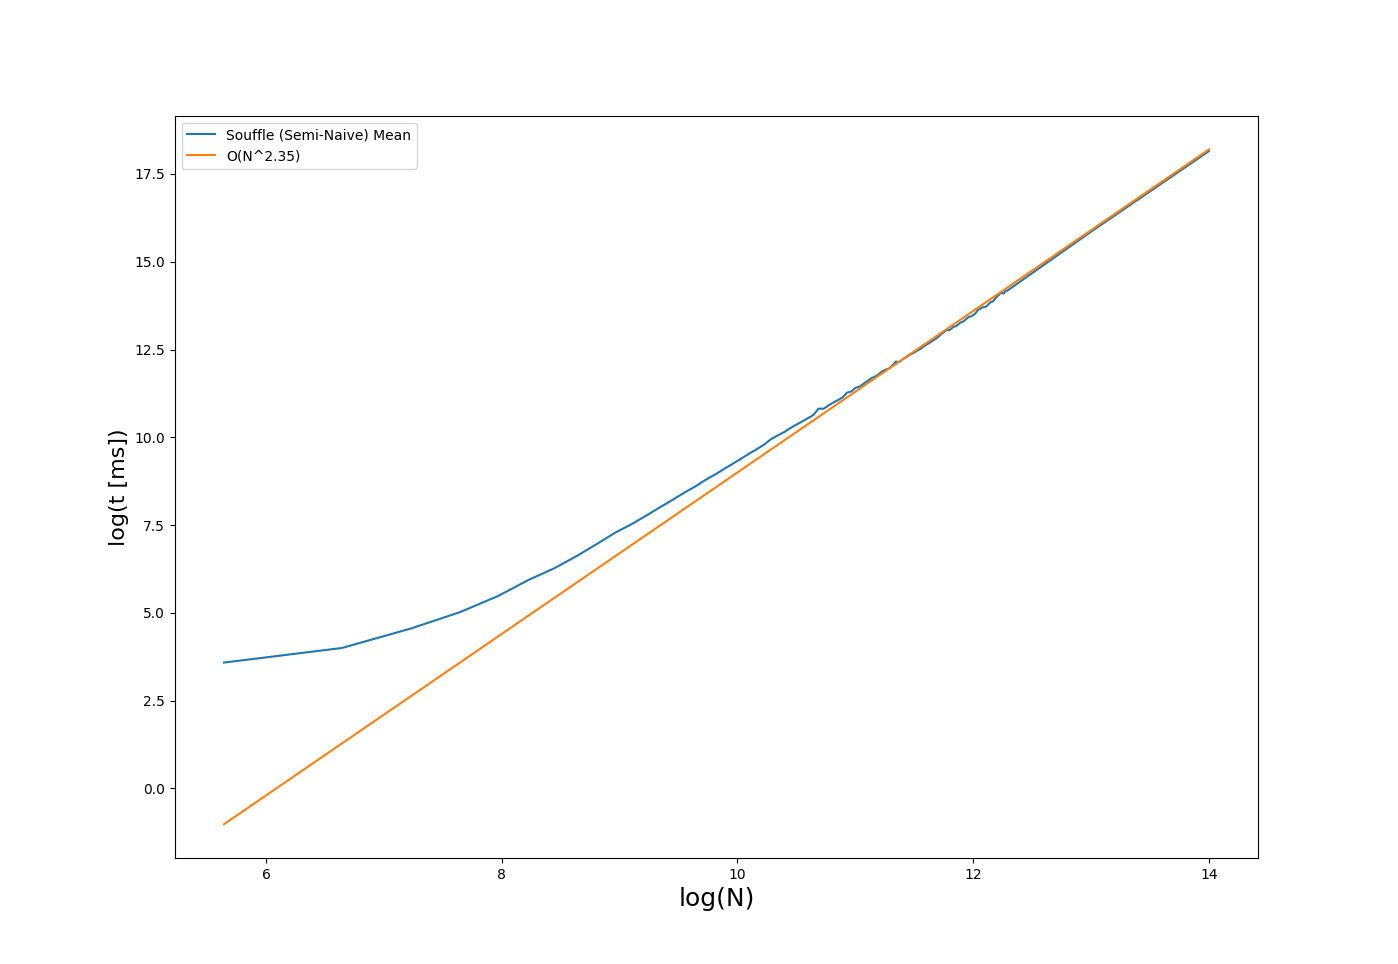
\includegraphics[scale=0.35]{img/ancestorSouffle.png}
%	\end{minipage}
%	\label{figure:ancestorExperimental}
%	\caption{Ancestor Example, \textbf{Left: } Internal (Naive), \textbf{Right: } Souffle (Optimized Semi-Naive)}
%\end{figure*}
\vspace*{-5pt}
\subsection{Expressive Power}
Souffle supports all the implemented language extensions except meta-predicates and type-inference\cite{SouffleHome}. The current set of meta-predicates offered by \datalogM does not extend the expressive power in any meaningful way, but rather permits more compact and (admittedly subjectively) more beautiful descriptions of Datalog programs. 

Souffle contains a number of language extensions that are not currently supported by \datalogM. For example, aggregate functions (such as $COUNT$, $MIN$, $MAX$), union types (i.e. stating that a term has type $A$ OR type $B$), and inbuilt functions (e.g. string operations), and more\cite{SouffleHome}.

